\chapter{用户体验的要素PPT中文模型}

\begin{center}
来源:\url{http://blog.rexsong.com/?p=11672}
作者:一叶千鸟\cite{The_Elements_of_User_Experience_cn}
\end{center}

最近狂做PPT,多次用到The Elements of User Experience的模型图。以前都是截图贴用,有三个问题,第一苦于无法插入动画在传达上大打折扣,第二因为受众原因肯定中文版更好,第三截图做的效果自然也一般。于是尝试用PPT搞了一个,基本上等比放大的中文版,效果还不错。网上能查到三个不同的中文版本,也都是图片,而且说实话做的不咋地。

我把五个层也加了上去,并稍微改了下传达形式,也提供了原版(颜色值均分毫不差)。压缩包里有PDF和PNG, PPT, PPTX四种格式,其中PPTX为PowerPoint 2010创建,规格为A4大小。PPTX格式内的图形可以直接拷贝编辑,也可以把PDF直接插入文档使用。

题外话,最近我们内部也在争论,主要是针对这个已经N年的模型图看是否有改进可能,当然本地化因素也在其中。在还没有新结论前,这个The Elements of User Experience模型的同行认可度(尤其海外)是最高的,个人认为只在“框架层”有些许不妥,其他都还OK,主要是普适性非常好,至少也不会误导人。
\bibliographystyle{plainnat}
\bibliography{gk}
\clearpage

\begin{figure}
\centering
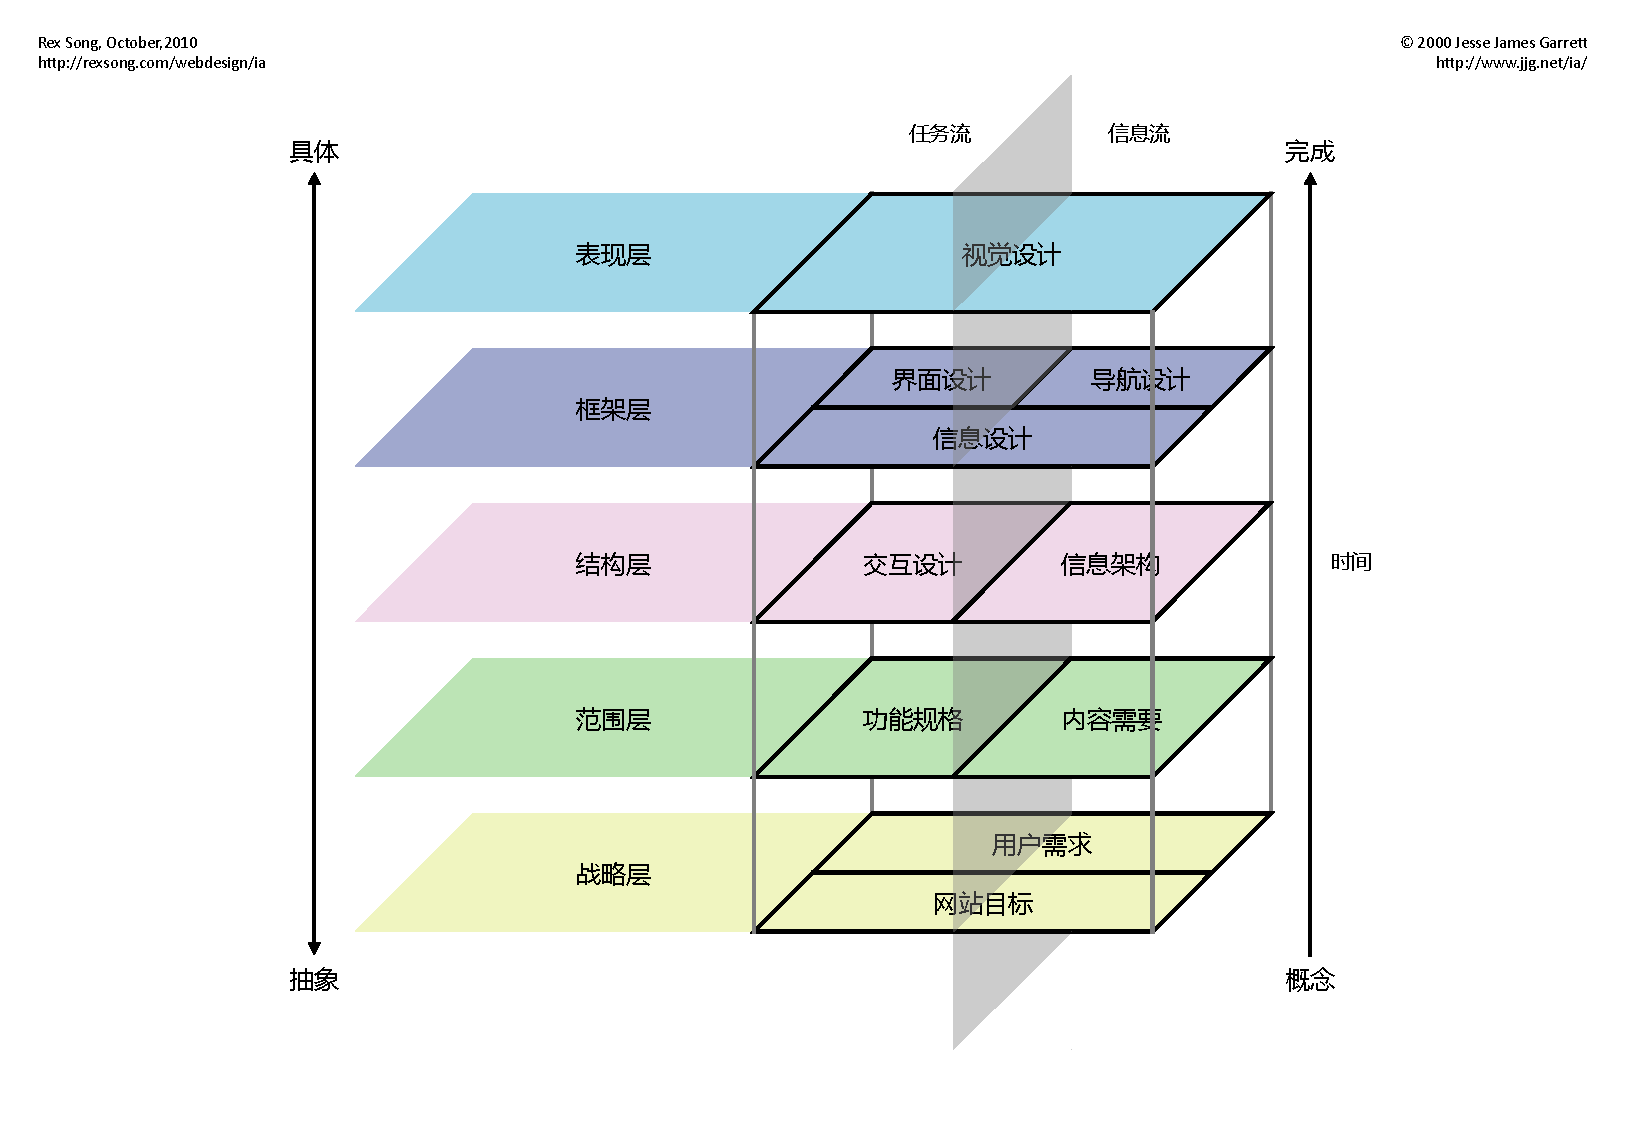
\includegraphics[scale=0.5]{model.pdf}\\
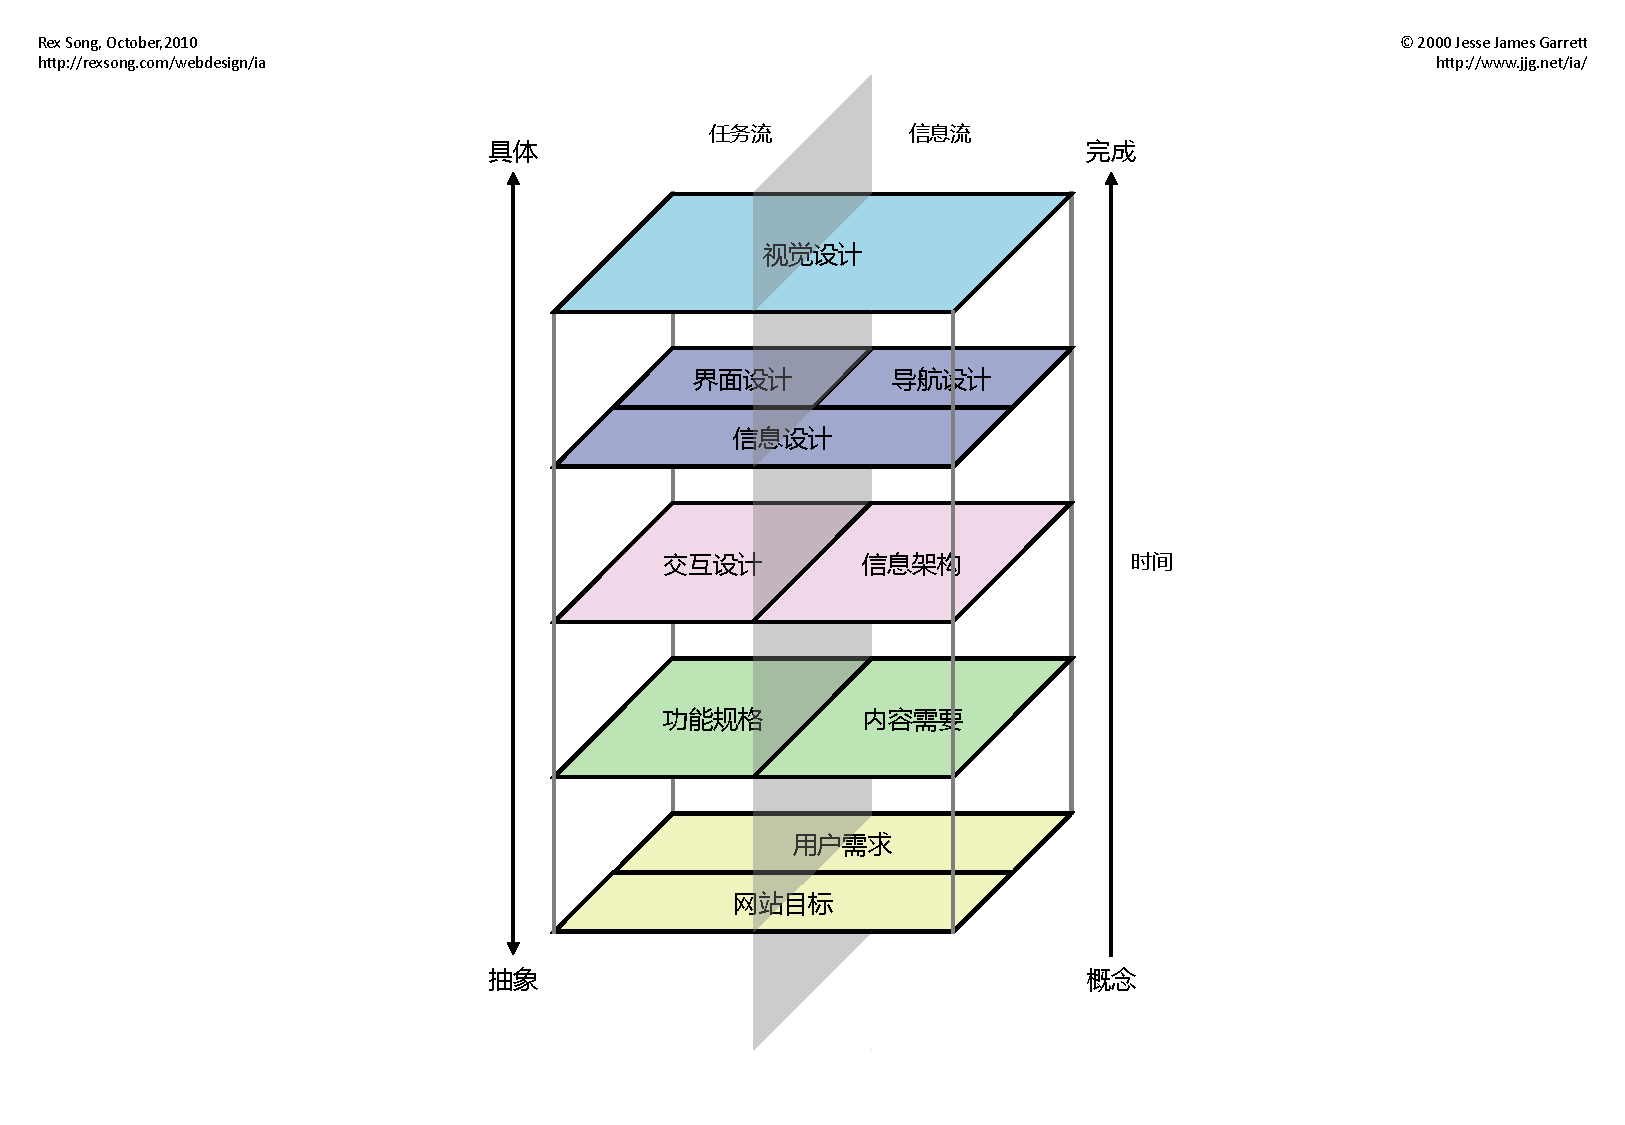
\includegraphics[scale=0.5]{models.pdf}
\end{figure}





